\begin{figure}[!htb]
	\begin{center}
		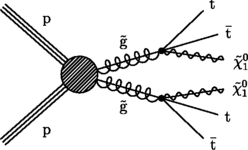
\includegraphics[width=0.32\textwidth]{T1tttt.png}
		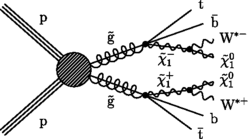
\includegraphics[width=0.32\textwidth]{T1ttbb.png} \\
		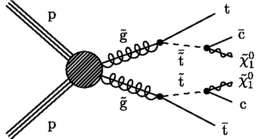
\includegraphics[width=0.32\textwidth]{T5ttcc.png}
		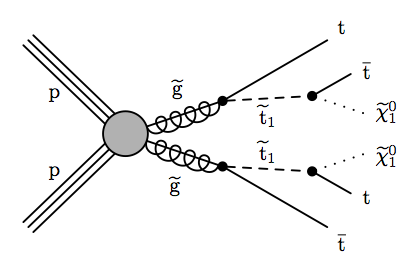
\includegraphics[width=0.32\textwidth]{T5tttt.png} \\
	\end{center}
	\caption[Gluino mediated stop production]{Feynman diagrams for the indirect \st{} production in SUSY. The allowed decay modes are T1tttt, T1ttbb, T5ttcc, and T5tttt.
	}
	\label{fig:stop-gluino-production}
\end{figure}

\begin{figure}[!htb]
	\begin{center}
		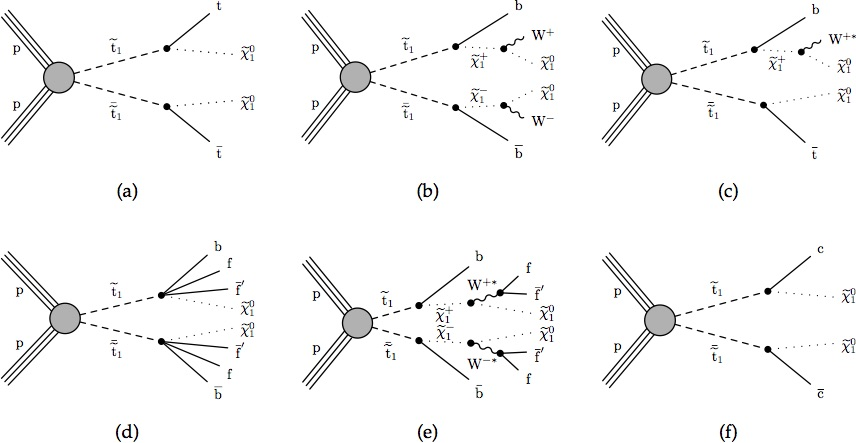
\includegraphics[width=1.00\textwidth]{T2tt_all.jpg}
	\end{center}
	\caption[Direct stop production]{Feynman diagrams for the direct \st{} production in SUSY. The allowed decay modes are T2tt, T2bW, T2tb, T2fbd, and T2cc. }
	\label{fig:stop-direct-production}
\end{figure}